\documentclass[a4paper,12pt]{article}
\usepackage{caption}
\usepackage{subcaption}
\usepackage{float}
\usepackage[T1]{fontenc}
\usepackage[italian]{babel}
\usepackage[utf8]{inputenc}
\input funzioni.sty
\input funzioni2.sty
\floatstyle{ruled}
\usepackage{hyperref}
\usepackage{graphicx}
\usepackage{amsmath}
\usepackage{amssymb}
\usepackage[width=125mm]{caption}
\usepackage{amsthm}
\usepackage{algorithm2e}
\usepackage{dsfont}
\usepackage{amsthm}
\usepackage{algpseudocode}
\usepackage{empheq}
\usepackage{tikz}
\usepackage{cancel}

% Dimensione della pagina
\setlength{\oddsidemargin}{.3in}  % Distance from the left edge -1 inch 
\setlength{\textwidth}{145mm}     % Normal width of the text
\setlength{\topmargin}{.25in}     % Distance from top to PAGE'S HEAD -1 inch
\setlength{\textheight}{225mm}    % Height of the body of page
\setlength{\headheight}{0mm}      % Height of a box containing the head
\setlength{\parskip}{0.5mm}         % Extra vertical space before a paragraph
\setlength{\parindent}{9mm}       % Width of the indentation 
\linespread{1.12}                 % Line spacing        
\renewcommand{\floatpagefraction}{.9}

\newtheorem{Teorema}{Teorema}

\begin{document}
\title{\bf \Huge Stuttura della Materia}

\author{Stefano Mandelli\\
	Dipartimento di Fisica, Universit\`a degli Studi di Milano,\\
	Via Celoria 16, 20133 Milano, Italia
}

\maketitle
\begin{center}
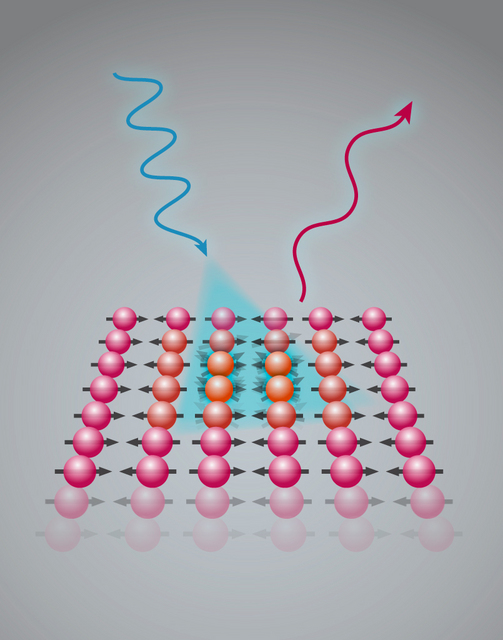
\includegraphics[scale=0.9]{IMG/copertina.jpg}
\end{center}

\newpage
\tableofcontents
\newpage

%----------------------------------------------------------------------------
\section{Particella in Campo Centrale}
%----------------------------------------------------------------------------
L'operatore che descrive il fenomeno sarà dato dalla parte cinetica e dalla parte di potenziale, che dipenderà in un qualche modo da $r$. In particolare 
\newl{\op{H} = \frac{1}{2m}\sum\op{p} ^2 + U\left(\sqrt{\sum x^2}\right).}
Definendo l'operatore \textit{Momento Angolare Orbitale} come
\newl{\op{L} _i = \varepsilon_{ijk}\op{x} _j \op{p} _k}
che in modo esplicito si scrive come
\newl{\op{L} _x = y p_z - z p_y \;\; ; \;\;  \op{L} _y = zp_x - xp_z \;\; ; \;\; \op{L} _z = xp_y - yp_x}
\begin{Teorema}
	Ogni operatore che può essere scritto nella forma $\ps{\op{v_1} }{\op{v_2} } $ commuta con $\op{L} $.
\end{Teorema}
\begin{proof}
\newl{\left[\op{L}, \op{v} _1\cdot \op{v} _2\right] &=& \sum_k \left[\op{L} _h, \op{v} _{1k} \right]\op{v} _{2k} + \sum_k \op{v} _{1k} \left[\op{L} _h, \op{v} _{2k} \right] = i\hbar\varepsilon_{hkl}\op{v} _{1l} \op{v} _{2k} + i\hbar\varepsilon_{hkl} \op{v} _{1k} \op{v} _{2l} =\nonumber \\ &=&i\hbar(\varepsilon_hkl + \varepsilon_{khl}) \op{v} _{1k} \op{v} _{2k} = 0 }
\end{proof}
In virtù di questo, si ottiene il risultato notevole
\newl{[\op{L} , \op{p} ^2] \;\; , \;\; [\op{L} , \op{v} ^2]}
Se due operatori essenzialmente autoaggiunti commutano tra loro, allora l'autospazio di uno è l'autospazio dell'altro. \footnote{Perlomeno... credo che dovrebbe essere così...}. In questo modo è possibile notare che $\op{L} $ commuta con l'Hamiltoniana di campo centrale $\op{H} = k \op{p} ^2 + f(\op{r} \cdot \op{r} )$
\newl{[\op{L} , \op{H} ] = [\op{L}, \op{p} ^2] + [\op{L} , f(\op{r} \cdot \op{r} )] = 0.}
Per sfuttare il lemma di Shur, si costruisce per praticità l'operatore $\op{L} ^2$ definito come
\newl{\op{L} \cdot \op{L} = \op{L} _x^2 + \op{L} _y^2 + \op{L} _z^2 = \op{L} ^2 .}
$\op{L} ^2$ commuta con $\op{L} _z$, quindi posso pensare di decomporre lo spazio di Hilbert negli autospazi di $\op{L} ^2$ e $\op{L} _z$. Seguendo la simmetria del problema riscrivo l'operatore $\op{L} ^2$ in coordinate sferiche
\newl{\op{L} ^2 = -\hbar^2 \left(\frac{1}{\sin\vartheta} \frac{\partial}{\partial\theta} \sin \vartheta \frac{\partial}{\partial \vartheta} + \frac{1}{\sin^2 \vartheta} \frac{\partial^2}{\partial \varphi ^2}\right) }
insieme all'operatore laplaciano
\newl{-\frac{\hbar^2}{2m}\Delta_2 = -\frac{\hbar^2}{2m}\frac{1}{r^2}\frac{\partial}{\partial r} r^2 \frac{\partial}{\partial r} + \frac{1}{2m r^2} \op{L} ^2 }
\subsection{L'autospazio di $L_z$}
Sfruttando le simmetrie del problema, posso trovare l'autospazio di $L_z$. Dato che commuta con $L^2$, che a sua volta commuta con l'Hamiltoniano, trovare l'autospazio di $L_z$ equivale trovare uno spazio in cui posso andare a cercare le autofunzioni di $\op{H} $. Presa una $f(r,\vartheta,\varphi)\in L^2(\R^3)$ continua e periodica nella variabile $\varphi$. Risolvo il problema agli autovalori dell'operatore $L_z$ che è definito come $L_z=-i\hbar \partial/\partial\varphi$
\newl{-i\hbar\frac{\partial}{\partial \varphi} f(r,\vartheta, \varphi) = \lambda f(r,\vartheta, \varphi).}
Fissando $r$ e $\vartheta$ ottengo un'equazione differenziale nella variabile $\varphi$ 
\newl{\frac{\partial}{\partial \varphi} \frac{f}{f(\varphi)} = \frac{i\lambda}{\hbar}.}
La soluzione è immediata
\newl{\log( f(\varphi) ) = \frac{i\lambda}{\hbar} \varphi \;\;\implicaa\;\; f(\varphi) = A\cdot e^{\frac{i\lambda}{\hbar} \varphi}   .}
Le autofunzioni di $L_z$ sono quindi del tipo
\newl{f(r,\vartheta,\varphi) = A(r,\vartheta) e^{\frac{i\lambda}{\hbar}\varphi} .}
Gli autovalori li ottengo imponendo le condizioni sull'angolo $\varphi$,
\newl{0\leq\varphi\leq 2\pi \;\;\implicaa \;\; e^{\frac{i\lambda 2\pi}{\hbar}}=1 }
la condizione su $\lambda$ diventa quindi
\newl{\lambda = \hbar m\;\;\;\;\; m \in N .}
Concludendo l'autospazio di $L_z$ è
\newl{S_m=\left\lbrace\frac{A(r,\vartheta)}{\sqrt{2\pi}}e^{im\varphi}\right\rbrace. }
Queste autofunzioni generano tutto lo spazio di Hilber e costuituiscono un s.o.n.c.
La somma ortogonale di tutti gli spazi $S_m$ genera tutto $L^2 (\R^3 )$ 
\newl{\oplus \sum_mS_m = L^2 (\R^3).}
In questo modo vale che $\forall f(r,\vartheta,\varphi) \in L^2(\R^3)$ è possibile scriverla sviluppata sulla base di $S_m$
\newl{f(r,\vartheta,\varphi) = \sum_{-\infty}^{+\infty} \frac{A(r,\vartheta)}{\sqrt{2\pi}} e^{im\varphi}}
dove le $A(r,\vartheta)$ sono funzioni t.c. $\int_{-\infty}^{+\infty}r^2\,dr\int_0^{2\pi}\sin\vartheta\abs{A(r,\vartheta)} \,d\vartheta<\infty$. Antitrasformando è possibile ricavare in modo formale le $A(r,\vartheta)$
\newl{A(r,\vartheta) = \int_0 ^{2\pi} \frac{1}{\sqrt{2\pi}} e^{-im\varphi'} f(r,\vartheta,\varphi') \,d\varphi'.}
La misura che faccio sull'osservabile $f$ può quindi essere vista come una proiezione dalle funzioni di $L^2(\R^3)$ sullo spazio di $L_z$. Questo viene definito come \textit{misura a valore di proiettore} e l'operatore che ne descrive il funzionamento è dato da
\newl{(\op{\mathds E} _{S_m}^{L_z} f)(r,\vartheta,\varphi) = \frac{A_m(r,\vartheta)}{\sqrt{2\pi}} e^{im\varphi} = \frac{1}{\sqrt{2\pi}}\int_0 ^{2\pi} e^{-im\varphi'} f(r,\vartheta,\varphi') \,d\varphi' .}
Se $f$ è un autostato di $L_z$ la sua rappresentazione è
\newl{(\op{L} _z f)(r,\vartheta,\varphi)= \sum_{m=-\infty}^{+\infty} \hbar m A(r,\vartheta) \frac{e^{im\varphi}}{\sqrt{2\pi}} = \sum_{m=-\infty}^{+\infty} \hbar m (\op{\mathds E} _{S_m}^{L_z} f)(r,\vartheta,\varphi)  }



\section{Fisica della Materia e della Radiazione}
Si definisce \textbf{Materia Condensata} un insieme di particelle interagenti. In funzione del numero di particelle, è possibile avere strutture differenti:
\begin{itemize}
	\item Nanostrutture $[\text{nm}]$ = caratterizzate da poche particelle interangeti, sul centinaio $(<10^3)$. Ovviamente avendo pochi atomi si hanno sttrutture molto piccole;
	\item Mesostrutture $[\mu m]$ = caratterizate da un numero di particelle di $\sim  10^4$;
	\item Strutture macroscopiche $[mm]$ = sono caratterizzate da un $N_A$ di particelle interagenti.
\end{itemize}
Lo scopo del fisico è quello di costruire modelli fisici partendo dall'osservazione. L'osservazione di un determinato fenomeno induce una domanda alla quale si cerca di rispondere attraverso la costruzione di un modello fisico. Davanti a questa necessità nasce il grande dilemma: quando usare un modello classico? Quando uno quantistico? La risposta varia di caso in caso. La descrizione di una particella, intesa come pacchetto d'onda, può cambiare molto in funzione al contesto in cui è inserita infatti se si ha sovrapposizione saranno presenti effetti quantistici che non si possono trascurare (per esempio l'interazione di scambio).

Se si considerano i pacchetti d'onda non sovrapposti in cui $p\gg (\Delta p)$ e  $V/N \gg (\Delta r)^3$ allora è possibile usare un modello classico rappresentato dalla lunghezza termica di De Broglie
\newl{\lambda_D=\frac{h}{p}=\frac{h}{\sqrt{2mE_C}} = \left(\frac{h^2}{3mK_BT}\right)^{\frac{1}{2}}}
con cui è possibile verificare che 
\newl{\frac{N}{V}\lambda_D^3 = \frac{N}{V}\left(\frac{h^2}{3mK_BT}\right)^{\frac{3}{2}}\ll 1.}
Si raggiunge la stessa conclusione partendo dal principio di indeterminazione di Heisenberg scritto nella ususale forma
\newl{\Delta r \cdot \Delta p \geq h.}
da cui è possibile ricavare
\newl{\frac{V}{N}p^3 \gg (\Delta r) \cdot (\Delta p) \geq h^3}
sapendo che $p=(3mK_BT)^{\frac{1}{2}}$ si ottiene nuovamente
\newl{\frac{N}{V}\left(\frac{h^2}{3mK_BT}\right)^{\frac{3}{2}}\ll 1.}
Un sistema può quindi essere modellizzato in modo classico per \textbf{densità} molto alte, \textbf{temperature} molto basse e \textbf{masse} molto piccole. Alcuni esempi sono dati da
\begin{itemize}
	\item Gas di idrogeno $[T\sim 0.26 K]$ sotto questa temperatura può essere modellizzato con le leggi classiche della cinetica dei gas;
	\item Elettroni di conduzione $[T \sim 1.8\cdot 10^5K]$ per modellizzare questo sistema è necessario usare modelli quantistici;
	\item Molti fotoni $(>10^3)$ si ha il campo elettromagnetico classico, quindi le equazioni di Maxwell;
	\item Pochi fotoni $(<10)$ si ha la QED (Quantum Elettro Dynamic).
\end{itemize}

\section{Richiamo sui solidi}
La materia che si presenta sotto il suo stato di \textit{solido} ha la caratteristica di essere completamente ordinata, gode di simmetria per alcuni angoli particolari e ci sono delle periodicità nella struttura. Sistemi solidi amorfi si conoscono per 0D (così detti \textit{quantum dot} ), 1D e 2D (così detti \textit{quantum well} come per esempio il grafene). Oltre ai sistemi amorfi ci sono i \textit{Quasi Cristalli}. Sono caratterizzati dall'avere simmetrie miste, per esempio parti con celle penatgonali miste a parte con simmetria sferica. Per osservare come la materia è aggregata, quali simmetrie sono presenti ed eventuali correlazioni le osservazioni che si possono fare riguardano le figure di diffrazione costruite facendo diffrangere radiazioni differenti. In funzione al passo del reticolo\footnote{E' vera questa cosa? C'è effettivamente una correlazione tra campione che voglio studiare e la relazione che scelgo per studiarlo? Credo proprio di sì.} si possono studiare diverse immagini di diffrazione costruite per esempio con raggi X($1 KeV \sim 10KeV$), con diffrazione di neutroni ($0,1 eV\sim 1 eV$) oppure strutture superficiali, diffrazione di elettroni ($100 eV$). A temperature prossime a quelle dell'ambiente ($T\sim 300K$) i neutroni hanno un loro momento magnetico. In questo modo, vedendo l'interazione tra i netroni e la mataria posso farmi un'idea sulle sue proprietà magnetiche. In conclusione, se devo studiare le proprietà magnetiche della materia uso neutroni a temperatura prossima a quella ambiente. 
\subsection{Reticolo di Bravais}
Un reticolo generico è possibile definirlo come 
\newl{\vet{R} = n_1 \vet{a} _2   + n_2 \vet{a} _2 + n_3 \vet{a} _3} 
in cui i vettori $\vet{a} _i$ non devono essere complanari. Il reticolo a nido d'ape, per esempio, non è un reticolo di Bravais perchè non è un gruppo puntuale.
bla bla bla (va aggiunta roba sui solidi)
\section{Teoria elementare della diffrazione}
Sia dato un certo sample da studiare come in Fig.~$\ref{Diff:1}$.
\begin{figure}
	\centering
	\label{Diff:1}
	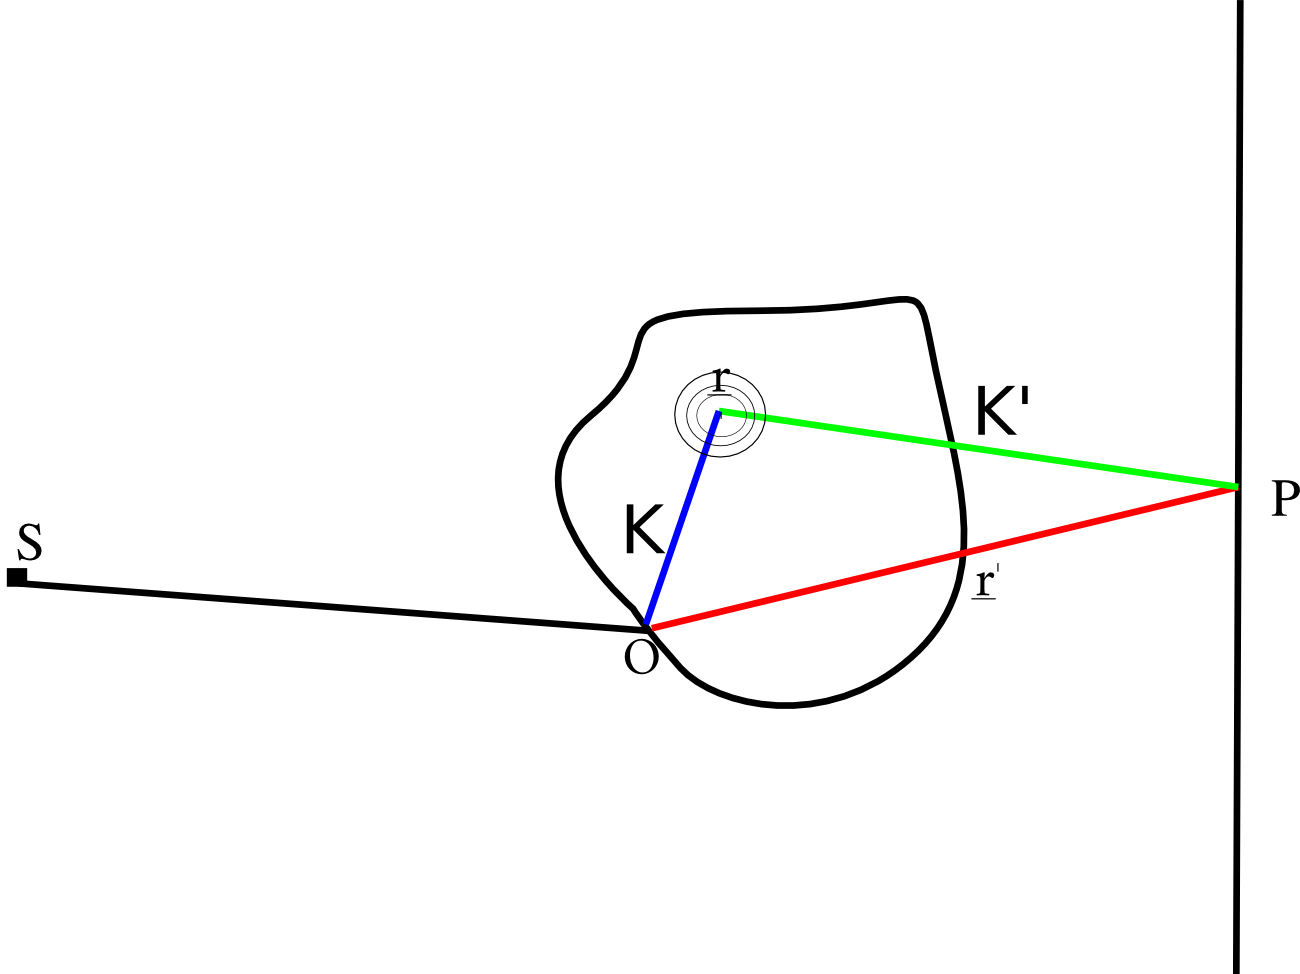
\includegraphics[width=120mm,angle=0,clip=]{IMG/Diff.png}
	\caption{Prova}
	\label{Diff:1}
\end{figure}
Supponendo $S$ una sorgente puntiforme e continua, la radiazione colpisce l'oggetto nel punto $\vec{r} $ che a sua volta diventa una sorgente di onde sferiche. Lo schermo si trova molto distante dall'oggetto colpito dalla radiazione, quindi $\abs{r'}  \gg \abs{r} $. La sorgente manda onde piane quindi
\newl{A(r)=A_Se^{i[k(r+R)-\omega t]}}
Si vuole evitare lo scattering multiplo considerando una singola interazione per ogni particella. L'onda interagisce con l'oggetto nel punto $r$ generando onde sferiche che raggiungeranno lo schermo e verranno viste nel punto $P$. Le onde diffratte avranno come vettore d'onda ${\vet k'} $. Quello che vedo nel punto $P$ sarà proporzionale a
\newl{A_P(r)=\int d^3r A(r)\rho(r)\left(\frac{e^{ik\cdot(r'-r)}}{|r'-r|}\right)}
dove $\rho(r)$ è la densità elettronica nel punto di interazione. Sviluppando l'espressione del potenziale nel punto $P$ e raggruppando tutti i termini indipendenti da $r$ ottengo
\newl{A_P(r) = \frac{A_Se^{i(k\cdot R + k'\cdot r' -\omega t)}}{|r'|} \int d^3r\rho(r)e^{-i(k'-k)\cdot r}.}
$A_P(r')$ è un integrale perchè va inteso come somma di tutte le onde piane generate dal punto $r$ di interazione della radiazione incidente con l'oggetto. Quello che interessa è l'intensità delle spot sullo schermo, quindi si deve considerare il modulo quadro
\newl{I_P(r)= \frac{|A_S|^2}{|r|^2}\left|\int d^3r \rho(r) e^{-i q\cdot r} \right|}
dove $\vet{q} = \Delta \vet{k} = \vet{k'} - \vet{k}$. Si può notare che $\int d^3r \rho(r) e^{-i q\cdot r}$ è la trasformata di fourire della $\rho(q)$, quindi posso scrivere:
\newl{I_P(\vet{q}) = \frac{|A_S|^2}{|\vet{r} |^2}\left|\op{\rho} (\vet{q}) \right|}
Dato che l'obiettivo è quello di ricavare le distribuzioni elettroniche e dato che sullo schermo compare l'immagine della trasformata di fourier delle distribuzioni, a rigor di logica, antitrasformando si dorebbero ottenere le $\rho(r)$. Questo non è possibile perchè l'evidenza sperimentale sullo schermo è data dal modulo quadro della trasfomata di Fourier, quindi mi manca il termine di fare per poter ricavare le distribuzioni nello spazio reale.

Per la trasformata di Fourier vale sempre che: $\Delta q_x \cdot \Delta x \sim \pi$ quindi si deve tenere in considerazione il fatto che per ottenere alte risoluzioni spaziali (quindi piccoli $\Delta x$) mi servono grandi momenti $p_x$.
\subsection{Reticolo Semplice}
\`E possibile applicare la teoria della diffrazione a modelli gradualmente sempre più complessi. Il primo modello che ci si presta ad affrontare è quello di un reticolo semplice. Il reticolo infatti è periodico con gli atomi vincolati nella loro posizione fissa. La distribuzione di carica elettronica è possibile quindi vederla espansa in serie di Fourier
\newl{\rho(\vet{r} )= \chi_V(\vet{r}) \sum_{\vet{G}} \rho_{\vet{G}} e^{i\vet{G} \cdot \vet{r}}.}
Trasformo e ottengo 
\newl{\op{\rho} (\vet{q})=\sum_{\vet{G}}\int_V \rho_{\vet{G}} e^{-i(\vet{G} - \vet{q} ) \cdot \vet{r}}.}
Possibili casi:
\begin{itemize}
	\item Se $\vet{G} \neq \vet{q}$: $\op{\rho} (\vet{q}) =0$;
	\item Se $\vet{G} = \vet{q}$ : $\op{\rho} (q) = V\rho_{G } \delta_{G ,q}$.
\end{itemize}
Quindi se $\vet{q}  = \vet{G} $ cioè $\vet{G} = \vet{\Delta k} = \vet{k'} - \vet{k}$ si hanno dei picchi, altrimenti il termine ${\vet G} - {\vet q}$ all'esponente dell'esponenziale complesso all'interno dell'integrale è molto grande. L'integrale di un esponenziale complesso, con argomento molto grande, ha media nulla, quindi non sono visibili picchi. La regola:
\newl{\boxed{\vet{G} = \vet{\Delta k} = \vet{k'} - \vet{k}}} 
viene chiamata \textbf{\textit{condizione di Von Laue}}. 
\begin{figure}
	\centering
	\fbox{
		\begin{tikzpicture}[scale=1,auto=center]
			\node[fill=none] (n1) at (-0.25,0) {O};
			\node (n2) at (4.25,2) {$\vet{k'}$};
			\node (n3) at (4.25,-2) {$\vet{k}$};
			\node (n4) at (4.25,0) {$\vet{q} $};
			\foreach \from/\to in {n1/n2}
			\draw [->] (0,0) coordinate (a) -- (4,2) ;%node[draw=none,fill=none,font=\scriptsize,midway,below] {text below};
			\foreach \from/\to in {n1/n3}
			\draw [->] (0,0) -- (4,-2) coordinate (b)  ;%node[draw=none,fill=none,font=\scriptsize,midway,below] {text below};		
			\foreach \from/\to in {n3/n2}
			\draw [->] (4,-2) -- (4,2) coordinate (c) ;%node[draw=none,fill=none,font=\scriptsize,midway,below] {$\vet{q} $ };
			\draw [->] (0,0) -- (5,0);
			\draw (1,0) arc (0:30:1);
			\draw (1,0) arc (0:-30:1);
			\node[] at (15:1.25)  {$\theta_{1}$};
			\node[] at (-15:1.25) {$\theta_{2}$};
		\end{tikzpicture}
	}
	\caption{Scattering totalmente elastico.}
	\label{bragg}
\end{figure}
Dalla Fig.\ref{bragg} è possibile dedurre la legge di Bragg in quanto, anche in questo caso, lo scattering radiazione-materia è di tipo totalmente elastico. Scrivendo la condiozine di Von Laue ottengo che
\newl{\vet{G} = \vet{q} = \Delta\vet{k} \implicaa \abs{G} = \abs{\Delta\vet{k}} }
considerando diffrazione per due piani paralleli:
\newl{\abs{G} = n\cdot \frac{2\pi}{d_{piani}}.}
Da Fig.\ref{bragg} si nota che a causa dello scattering completamente elastico si ha che $\theta_1 = \theta_2 = \theta$ quindi  $\abs{{\vet q} } = 2\abs{\vet{k} } \sin\theta$. Unendo le due precedenti riscritture del vettore $\vet{G}$ otteniamo la legge di Bragg
\newl{\boxed{\frac{4\pi\sin\theta}{\lambda} = n\frac{2\pi}{d_{piani}} \implicaa n\lambda = 2d\sin\theta . }}
Rimane ancora il fatto che se ${\vet q} ={\vet G}$ allora l'integrale ha dimensione di un $\rho_G \cdot V \delta_{{\vet q},{\vet G}} $ quindi l'intesità dell'immagine che vediamo sullo schermo risulta proporzionale a $I({\vet q}) \sim |\rho_G|^2 V^2 \delta_{{\vet q},{\vet G}}$. Non può essere proporzionale a $V^2$ è fisicamente impossibile in quanto la scrittura non torna dimensionalmente. La questione si risolve capendo che la funzione $\rho_G$ non è una funzione puntuale, ma ha una forma a spot di tipo campana gaussiana con piccole code. Effettuando l'integrale
\newl{\op{\rho} (\vet{q}) = \sum_G \int_V d^3r \rho_G e^{i(\vet{G}-\vet{q})\vet{r}}} 
è possibile arrivare ad un risultato che vede $I(\vet{q})\sim V$ che è fisicamente coerente.
\subsection{Un esempio più complesso: reticolo con base}
Un esempio più complesso può essere rappresentato dalla caratterizzazione dell'immagine di diffrazione da parte di un cristallo più complesso in cui abbiamo la sua rappresentazione tramite un reticolo e una base atomica. Il modo migliore per separare il problema è rappresentato in Fig.\ref{base:laue}.
\begin{figure}
	\centering
	\fbox{
		\begin{tikzpicture}[scale=1,auto=center]
			\draw [black] plot [smooth cycle] coordinates {(-1.5,-2.5) (-1,6) (5,6) (7,6) (7.5,4) (7,3) (6,-2)};
			\draw [->] (-1.5,-2.5) -- (0,0);
			\node (n1) at (-1,-1) {$\vet{R_n} $};
			\node (n2) at (0.25,0.45) {$\vet{r_\alpha} $};
			\draw [->] (0,0) -- (0.7,0.3);
			\draw (1,0.3) arc (0:360:0.3);
			\draw [->] (0.7,0.3) -- (0.7,0.6);
			\node (n3) at (0.9,0.65) {$\vet{r'} $};
			\draw [->] (-1.5,-2.5) -- (0.7,0.6);
			\node (n4) at (0,-1) {$\vet{r}$};


			\node[]  at (-1.7,-2.7) {O};
			\draw  (0,0) -- (4,0);
			\draw  (0,1) -- (4,1);	
			\draw  (0,2) -- (4,2);
			\draw  (0,3) -- (4,3);
			\draw  (0,4) -- (4,4);

			\draw  (0,0) -- (0,4);
			\draw  (1,0) -- (1,4);	
			\draw  (2,0) -- (2,4);
			\draw  (3,0) -- (3,4);
			\draw  (4,0) -- (4,4);

			\draw  (4,4) -- (6,5);
			\draw  (4,0) -- (6,1);
			\draw  (0,4) -- (2,5);

			\draw  (2,5) -- (6,5);
			\draw  (6,5) -- (6,1);

		\end{tikzpicture}
	}
	\caption{Sistema di riferimento di un cristallo complesso rappresentato da reticolo e base atomica.}
	\label{base:laue}
\end{figure}
Si prenda come origine un punto sul bordo dell'oggetto di forma generica. Il vettore $\vet{R}_n$ identifica la cella cristallina, il vettore $\vet{r}_\alpha$ identifica l'atomo $\alpha-esimo$ della base nella cella ed infine il vettore $\vet{r'}$ identifica la nuvola elettronica intorno all'$\alpha-esimo$ atomo. \`E  quindi possibile scrivere che
\newl{\boxed{\vet{r}=\vet{R}_n + \vet{r}_\alpha + \vet{r'}}.} Ovviamente $\vet{r}$ identifica un punto della nuvola elettronica dei vari $\alpha$ atomi che costituiscono la base della cella cristallina. Nell'integrale entra appunto solo il contributo delle nuvole elettroniche in quanto noi stiamo usando raggi $X$ che interagiscono con le nuvole elettroniche degli atomi. Calcoliamo in questo caso come è fatta l'immagine di diffrazione del cristallo passando sempre per la trasformata di Fourier della distribuzione di carica
\newl{\op{\rho} (\vet{q}) &=& \int_V d^3r\, \rho(\vet{r})e^{-i\vet{q}\cdot \vet{r}} = \sum_{n_1,n_2,n_3}\sum_{\alpha} \int_Vd^3r'\,\rho_\alpha e^{-i\vet{q}\cdot(\vet{R}_n + \vet{r}_\alpha + \vet{r'})}= \nonumber\\
			  &=&\sum_{n1,n2,n3} e^{-i\vet{q}\cdot\vet{R}_n} \sum_\alpha e^{-i\vet{q}\vet{r}_\alpha} \int_{V_{cella}} d^3r'\,\rho_\alpha(\vet{r}')e^{-i\vet{q}\cdot\vet{r'} }
}
in questo modo tutto si riduce all'integrale sul volume della $\rho(r')$ elettronica del singolo atomo. L'intensità è data sempre dal modulo quadro quindi è possibile scrivere
\newl{\boxed{I(\vet{q})=\overbrace{ \abs{\sum_{n1,n2,n3} e^{-i\vet{q}\cdot\vet{R}_n}} ^2 }^{\text{Fattore di Interferenza}} \overbrace{\abs{\sum_\alpha e^{-i\vet{q}\vet{r}_\alpha} \int_{V_{cella}} d^3r'\,\rho_\alpha(\vet{r}')e^{-i\vet{q}\cdot\vet{r'} } } ^2 }^{\text{Fattore di Struttura}} }.}
Il Fattore di interferenza è diverso da zero solo per ${\vet q} = {\vet G}$ quindi, questa condizione, determina in che posizione avvengono i picchi. Il fattore di struttura, è quella parte che contribuisce all'allargamento del picco e rappresenta la trasformata di Fourier della densità elettronica dell'atomo $\alpha$ sulla cella. Questa parte è nota come \textit{Fattore di Forma Atomico}.
\begin{figure}
	\centering
	\fbox{
		\begin{tikzpicture}[scale=1,auto=center]
			\draw [->] (-1,0) -- (7,0);
			\draw [->] (0,-1) -- (0,7);
			\node (n1) at (7,-0.25) {${\vet q}$};
			\node (n2) at (-0.5,7) {$I({\vet q})$};
			\node (n3) at (1,-0.25) {${\vet G_1}$};
			\node (n4) at (2,-0.25) {${\vet G_2}$};
			\node (n5) at (3,-0.25) {${\vet G_3}$};
			\node (n6) at (4,-0.25) {${\vet G_4}$};
			\node (n7) at (5,-0.25) {${\vet G_5}$};
			\node (n8) at (6,-0.25) {${\vet G_6}$};

			\draw [red] plot [smooth, tension=0.2] coordinates {(0.5,0) (0.7,0.25) (1,4) (1.3,0.25) (1.5,0)};
			\draw [red] plot [smooth, tension=0.2] coordinates {(1.5,0) (1.7,0.25) (2,4) (2.3,0.25) (2.5,0)};
			\draw [red] plot [smooth, tension=0.2] coordinates {(2.5,0) (2.7,0.25) (3,4) (3.3,0.25) (3.5,0)};
			\draw [red] plot [smooth, tension=0.2] coordinates {(3.5,0) (3.7,0.25) (4,4) (4.3,0.25) (4.5,0)};
			\draw [red] plot [smooth, tension=0.2] coordinates {(4.5,0) (4.7,0.25) (5,4) (5.3,0.25) (5.5,0)};
			\draw [red] plot [smooth, tension=0.2] coordinates {(5.5,0) (5.7,0.25) (6,4) (6.3,0.25) (6.5,0)};

			\draw [green] plot [smooth, tension=1] coordinates {(-0.5,5) (3.5,5.7) (6.5,5)};

			\draw [green] plot [smooth, tension=0] coordinates {(4,7) (4.6,7)};
			\draw [red] plot [smooth, tension=0] coordinates {(4,6.5) (4.6,6.5)};

			\node[] at (6,7) {\fontsize{1mm}{1mm}\selectfont Fattore di Struttura};
			\node[] at (6,6.5){\fontsize{1mm}{1mm}\selectfont Fattore di Interferenza};
		\end{tikzpicture}
	}
	\caption{Fattore di Interferenza e Fattore di Struttura}
	\label{str:int}
\end{figure}
In Fig.\ref{str:int} sono rappresentati i contributi dei fattori di interferenza e struttura. Come è possibile osservare il fattore di interferenza è rappresentato da dei picchi situati in prossimità dei vettori $ {\vet G_n}$ e identificano le $N$ celle del reticolo cristallino.
\subsection{Un Liquido}
Supponiamo di indebolire il fatto che il reticolo sia cristallino. Supponiamo di avere a che fare con un oggetto che abbia le caratteristiche di un fluido. In questo caso fisso un ${\vet R} _n$ e sommo su tutti i vari ${\vet R} _m$. Devo quindi avere una funzione di correlazione spaziale che mi permetta di sapere in che posizione sono i vari ${\vet R} _m$ ripetto al mio punto fisso ${\vet R} _n$. Il fattore di interferenza diventa quindi 
\newl{T({\vet q}) &=& \abs{\sum_{n_1,n_2,n_3} e^{-i{\vet q} \cdot{\vet R}_n } }^2 = \sum_{{\vet R}_m = {\vet R}_n} e^{-i{\vet q}\cdot({\vet R}_n -{\vet R}_m)}+ \sum_{{\vet R} _n \neq {\vet R} _m } e^{-i{\vet q} \cdot({\vet R} _n- {\vet R} _m)} = \nonumber\\ &=& N + \sum_{{\vet R_n}} \left(\sum_{{\vet R} _n \neq {\vet R} _m}e^{-i{\vet q}(\vet{R} _n - {\vet R} _m)} \right) }
Estendo al continuo
\newl{T(\vet{q}) &=& N + N\int d^3r\, e^{-i{\vet q}\cdot(R_n-R_m)}P(R_n-R_m) = \nonumber\\
			       &=& N\left(1+\int d^3r\, e^{-i{\vet q}\cdot(R_n-R_m)}P(R_n-R_m)\right) 
}
Dove $P(R_n-R_m)$ è la funzione di correlazione spaziale che permette di studiare strutture non perfettamente regolari.

\section{Elettroni nel potenziale periodico}
Il problema agli autovalori che bisogna risolvere per trattare eletroni liberi in un potenziale periodico è il tipico
\newl{\left[-\frac{\hbar^2}{2m}\nabla^2 +U_e({\vet r})\right]\psi_n({\vet r}) = E_n \psi_n({\vet r}),}
dove si stanno facendo le seguenti approssimazioni:
\begin{itemize}
	\item Elettroni \textbf{indipendenti};
\end{itemize}
In questo modo la funzoine d'onda che descrive il problema è possibile fattorizzarla.
\begin{itemize}
	\item Il potenziale è periodico, quindi $U({\vet r}  + {\vet R} )  = U({\vet r}  )$
\end{itemize}
Il teorema di Bloch mi dice che per un potenziale periodico la funzoine d'onda è possibile fattorizzarla come una parte di onda piana e una parte periodica
\newl{\boxed{\psi_{n,\vet{k}}(\vet{r})=\overbrace{e^{i\vet{k}\cdot\vet{r}}}^{\text{Onda Piana}} \overbrace{u_{n,\vet{k}}(\vet{r}) }^{\text{Periodica}}}}
\subsection{Giustificazione fisica del teorema di Bloch}
La giustificazione del teorema di Bloch e quindi della forma delle funzioni d'onda dell'elettrone libero all'interno di un cristallo, trova la sua base sulle ipotesi fatte appunto sul reticolo del cristallo stesso. E' tutto periodico quindi mi aspetto che i moduli quadri della funzione d'onda siano periodici con passo quello del reticolo cristallino
\newl{\abs{\psi(r)} ^2 = \abs{\psi(r+R)} ^2,}
in questo modo, la funzione d'onda avrà una sua certa parte radiale con un certo coefficiente $C_{\vet k}$ per cui deve valere il fatto che $\abs{C_k} =1$. Un modo molto conveniente che ho di vedere questa cosa è quella di pensare appunto il coefficiente $C_{\vet k}$ dato da un'onda piana, infatti, cercando l'ugualianza tra le parti radiali di $\psi_k(r)$ r $\psi_k(r+R)$, notiamo che:
\newl{e^{ikr}\left[e^{-ikr} u_{n,k}(r)\right] = e^{ikr}e^{ikR} \left[ e^{-ikr}e^{-ikR}u_{n,k}(r+R)\right]}
da cui
\newl{\boxed{u_{n,k}(r) = u_{n,k}(r+R) }.}
In questo modo si vuole dare una giustificazione molto intuitiva del perchè le funzioni d'onda del teorema di Bloch sono funzioni d'onda sensate che seguono bene le condizioni di periodicità del nostro problema. Le soluzioni dell'hamiltoniana sono in funzione alle condizioni al bordo che scegliamo. In questo caso ha perfettamente senso scegliere delle condizioni al bordo periodiche. La restrizione sui valori di $\vet k$ sarà data da una serie di considerazioni. Partendo dalla periodicità $\psi(r) = \psi(r+L)$ sul reticolo, quindi se $a$ è un vettore del reticolo diretto si ha che $L = Na$. uguagliando le funzioni d'onda
\newl{e^{ikx} = e^{ik(x+L)} u_k(x+L)} 
ho come condizione
\newl{\boxed{kL = n 2\pi\implicaa k=\frac{2\pi}{L}n\,\,\, \text{ dove } \,\,\,n\in\Z }}
questa appena scritta è la famosa condizione periodica di \textit{\textbf{Born - Von Karman}}. Dal punto di vista dello spazio dei vettori $\vet k$ questo vuol dire che tutto quello che succede nello spazio può essere rimappato nell'intervallo di $k\in\left[-\frac{\pi}{a},\frac{\pi}{a}\right]$ che è appunto la prima zona di Brillouin. Nello spazio $k$ posso verificare facilmente che $k = k'-G$ dove $G$ è un vettore di base del reticolo reciproco
\newl{\psi_{k'}(x)e^{ik'x}u_{k'}(x) = e^{i(k+G)x}u_{k+G}(x)= e^{ikx}\overbrace{e^{iGx}u_{k+G}(x)}^{\text{Sono periodiche}}= e^{ikx}\op{u_k} (x).} 
In questo modo abbiamo confermato quanto detto prima. Ongi vettore $k'$ può essere rimappato all'interno della prima zona di Brillouin.
\subsection{Formazione delle bande}
Supponiamo di essere in condizione di potenziale debole a media nulla e che valgano le condizioni al bordo elencate precedentemente. Possiamo quindi trattare il problema agli autovalori come particella libera a cui viene successivamente inserito il contributo del potenziale debole in modo perturbativo. Il punto di partenza è banalmente la particella libera
\newl{\left(-\frac{\hbar^2}{2m}\nabla^2\right)  \psi_k(r) = E \psi_k(r).}
Con le condizioni al bordo periodiche, l'energia in funzione di $\vet k$ ha la tipica dipendenza quadratica
\newl{E=\frac{\hbar^2}{2m}k^2.}
\begin{figure}
	\centering
	\fbox{
		\begin{tikzpicture}[scale=1,auto=center]
			%\draw [help lines] (0,0) grid (2,2);
			\draw [->] (-5,0) -- (5,0);
			\draw [->] (0,-2) -- (0,5);
			\draw (-4,0.3*4^2) parabola bend (0,0) (4, 0.3*4^2);
			\draw (-2,0.3*4^2) parabola bend (2,0) (5, 0.3*3^2);
			\draw (-5,0.3*3^2) parabola bend (-2,0) (2, 0.3*4^2);
			
			\draw (0,0.3*4^2) parabola bend (4,0) (5, 0.3*1^2);
			\draw (-5,0.3*1^2) parabola bend (-4,0) (0, 0.3*4^2);
			\draw[domain=-1:1, ultra thick] plot (\x,{0.3*(\x)^2+1.2*\x+1.2});
			\draw[domain=-1:1, ultra thick]  plot (\x,{0.3*(-\x)^2+1.2*(-\x)+1.2} );
			\draw[domain=-1:0, ultra thick]  plot (\x,{0.3*(\x+2)^2+1.2*(\x+2)+1.2} );
			\draw[domain=0:1, ultra thick]  plot (\x,{0.3*((-\x)+2)^2+1.2*((-\x)+2)+1.2} );

			\draw[ultra thick] (-1,0.3) parabola bend (0,0) (1,0.3);
			\draw[ultra thick] parabola (-1,0.3) (1,9*0.3);	


			\node[fill,thick,circle, inner sep=0pt, minimum size=0.2cm] at (1,0.3)  {};
			\node[fill,thick,circle, inner sep=0pt, minimum size=0.2cm] at (1,9*0.3)  {};
			\node[fill,thick,circle, inner sep=0pt, minimum size=0.2cm] at (-1,0.3)  {};
			\node[fill,thick,circle, inner sep=0pt, minimum size=0.2cm] at (-1,9*0.3)  {};



			\node[] at (1.25,0.3)  {$1$};
			\node[] at (1.25,9*0.3)  {$2$};
			\node[] at (-1.25,0.3)  {$3$};
			\node[] at (-1.25,9*0.3)  {$4$};

			\node[fill,thick,circle, inner sep=0pt, minimum size=0.1cm] at (1,-0) {};
			\node[fill,thick,circle, inner sep=0pt, minimum size=0.1cm] at (-1,0)  {};
			\node[] at (1,-0.4) {$\frac{\pi}{a}$};
			\node[] at (-1,-0.4)  {$-\frac{\pi}{a}$};

			\draw[] (-1,0) -- (-1,5);
			\draw[] (1,0) -- (1,5);
		\end{tikzpicture}
	}
	\caption{Ritratto in fase dei momenti di particella libera}
	\label{Part:Lib}
\end{figure}
In Fig.\ref{Part:Lib}, è ben visibile che non vi è separazione tra le bande. \`E possibile passare in modo continuo da una banda all'altra nei punto in cui il vettore d'onda interseca la zona di Brillouin. in questo modo i punti $1,2,3,4$ hanno livelli quasi-degeneri, con energie di bande diverse che risultano molto vicine per lo stesso valore di $\vet k$. Si può passare ora a studiare il modo in cui il potenziale debole $U_e$ agisce sui livelli energetici. Il potenziale è riferito ad un reticolo diretto con una sua certa periodicità, è possibile rappresentarlo in serie di Fourier rispetto ai vettori $\vet q$ del reticolo reciproco 
\newl{U_e(x) = \sum_q U_q e^{i{\vet q}\cdot {\vet x}}\,\,\,\,\,\,\,\, \left(q=\frac{2\pi}{a}m\right).}
Adottando la convenzione di fissare la scala delle energie sul valor medio del potenziale allora si ottiene che $U_0=0$. Questo semplifica in modo essenziale gli sviluppi perturbativi. Riscrivendo l'equazione di Schroedinger con il contributo del potenziale
\newl{\left[-\frac{\hbar^2}{2m_e}\nabla^2+U_e(x)\right]\psi(x)=E\psi(x).}
A questo punto è necessario fare alcune considerazioni sulla funzione d'onda: essa può essere rappresentata sul sistema o.n.c delle onde piane, con opportuni coefficienti $C_k\in\C$
\newl{\psi(x)=\sum_kC_ke^{ikx}.}
Inserendo la funzione d'onda nell'equazione di Schroedinger appena scritta si ottiene il seguente problema agli autovalori
\newl{\sum_k\left[-\frac{\hbar^2}{2m_e}(-k^2)C_ke^{ikx}\right]+\sum_{q,k}U_qC_ke^{i(q+k)x}=E\sum_kC_ke^{ikx}}.
Moltiplicando per $e^{ik'x}$ ed integrando, si ottiene il seguente sistema per i coefficienti $C_k$
\newl{\left(\frac{\hbar^2}{2m_e}k^2 -E\right)C_k + \sum_q U_qC_{k-q} =0.}
Dall'ultima scrittura è possibile notare che il termine di potenziale è responsabile dell'accoppiamento tra i vari coefficienti $C_k$ infatti mette in realazione ogni coefficiente relativo ad un vettore $\vet k$ ad suo rispettivo nelle altre zone di Brillouin (che differenziano appunto di un vettore $\vet q$). Dato che può essere rimappato tutto nella prima zona di Brillouin, questo vuol dire che il termine di potenziale aggiunge accoppiamento tra i vari termini dello sviluppo. Tra i vari $\vet k$ vettori della prima zona di Brillouin si immagini di fissarne uno. In corrispondenza si avranno autofunzioni e autovalori indicizzati $\vet k$. Le funzioni d'onda dovranno essere la sovrapposizione di tutte le onde piane che distano di un vettore $\vet q'$ perchè come detto prima tutto viene rimappato nella prima zona
\newl{\psi_k(x)=\sum_{q'}C_{k-q'}e^{i(k-q')x}.}
Si noti che la somma è solo sui $\vet q'$ quindi è possibile riscrivere la funzione d'onda come
\newl{\psi(x)=e^{ikx}\sum_{q'}C_{k-q'}e^{-iq'x} = e^{ikx}u_k(x),}
questa forma è la stessa indicata per funzioni d'onda di elettrone libero in un potenziale cristallino dal teorema di Bloch. Questo fatto, con una certa forzatura, è possibile interpretarlo comeun'ulteriore prova a favore del teorema di Bloch. Prendendo la funzione d'onda appena scritta e usandola nell'equazione di Schroedinger si ottiene
\newl{\sum_{q'}\left[\frac{\hbar^2}{2m_e}(k-q')^2C_{k-q'}e^{i(k-q')x}\right]+\sum_{q',q"}U_{q"}C_{k-q'}e^{i(q"+k-q')x}=E_k\sum_kC_{k-q'}e^{i(k-q')x}}
Sfruttando nuovamente l'ortonormalità delle onde piane e integrando su $q"$ si ottiene, per ogni valore di $\vet k$, un sistema di equazioni accoppiate
\newl{\left[\frac{\hbar^2}{2m_e}(k-q)^2 -E_k\right]C_{k-q} +\sum_{q'}U_{q'-q}C_{k-q'}=0}
che una volta risolto fornisce i livelli energetici e i coefficienti dello sviluppo in serie della funzione d'onda. Ponendo $U_q=0$ si ritorna al caso precedente di particella libera
\newl{E_k,q = E(k-q)=\frac{\hbar^2}{2m_e}(k-q)^2}.
In questo caso $\vet q$ rappresenta il numero quantico che identifica la banda. Se ${\vet k} \sim {\vet q} /2$ si è in una condizione quasi degenere. Per valori di $\vet k$ lontani da questi punti le bande sono ben separate, il problema è solo in prossimità di questi punti. Per il calcolo della correzione dell'energia per mezzo di un potenziale debole è necessario considerare i due casi in modo separato e non si può effettuare una trattazione perturbativa standard. \`E possibile verificare che nel caso degenere per le due bande $q$ e $q'$ si ha 
\newl{\boxed{\Delta E=\abs{E(k-q)-E(k-q')}  \ll U .}}
Essendo la correzione dell'energia proporzionale a $U$  è quindi molto più significativa del caso non degenere in cui $\Delta E\gg U$ e la correzione di energia è proporzionale a $U^2$ quindi totalmente trascurabile. Ha quindi senso studiare solo la correzione dell'energia per il caso degenere poichè solo in questo caso si prevedono modifiche consistenti ai livelli energetici.
Per due bande degeneri generiche $\vet q_1$ e $\vet q_2$, tenendo conto solo dei termini dominanti si ottiene il seguente sistema algebrico
\newl{\left[E-E_{k,q_1}\right]C_{k-q_1} = U_{q_2-q_1}C_{k-q_1} \nonumber\\
	\left[E-E_{k,q_2}\right]C_{k-q_2} = U_{q_1-q_2}C_{k-q_2}
}
Soluzioni non nulle per i coefficienti dello sviluppo della funzione d'onda si hanno se si annulla il determinante della matrice
\[ \left| \begin{array}{cc}
E-E_{k,q_1} & -U_{q_2-q_1}  \\
-U_{q_1-q_2} & E-E_{k-q_2} \end{array} \right|.\]
Risolvendo per $E$ e osservando che $U_{q_1-q_2} = U^*_{q_2-q_1}$ (a causa del fatto che il potenziale è una funzione reale), si ottiene la correzione all'energia
\newl{\boxed{E(k)=\frac{E_{k,q_1}+E_{k,q_2}}{2}\pm \frac{1}{2}\sqrt{(E_{k,q_1}-E_{k,q_2})^2 + 4\abs{U_{q_1-q_2}} ^2 }   }.}
Questo indica che intorno a $(q_1+q_2)/2$ i livelli energetici di elettrone libero sono molto vicini e diventa molto singificativo il contributo del termine di potenziale. I livelli si \textit{respingono} dando vita ad un \textbf{gap di energia}, ovvero ad una zona di energie proibita. Possiamo notare che le correzioni all'energia diventano quindi sensibili quando $\abs{k-q_1} ^2 = \abs{k-q_2} ^2$ cioè quando siamo in una zona di quasi degenerazione. Posso ridefinire ${\vet k'} = \vet k - \vet q_1$ e $\vet q = \vet q_1 - \vet q_2$ in questo modo posso riscrivere la condizione di quasi degenerazione come
\newl{\abs{\vet k'} = \abs{{\vet k} - {\vet q}} }
cioè 
\newl{\boxed{\Delta{\vet k} = {\vet q}}}
che è la condizione di diffrazione di Von Laue. Quindi si spiega il motivo per il quale le bande si aprono in prossimità di quei punti, gli elettroni non possono stare in quelle posizioni e vengono diffratti.
\subsection{Soluzione elettrone libero in un potenziale periodico}
Nel paragrafo precedente sono stati elencati una serie di riusltati sulla formazione dei gap energetici in corrispondenza dei punti di quasi degenerazione. E' stato possibile verificare che la correzione all'energia è sensibile solo in questi punti. Lontani dai punti di quasi degenerazione la correione all'energia diventa di ordine $O(N^2)$ quindi totalmente trascurabile. Per completare il concetto viene presentata, in modo più formale, la correzione agli autovalori per un elettrone libero in un potenziale periodico debole. Si consideri un potenziale realistico del tipo
\newl{V(x)=\sum_n v(x-na).
\label{PER:POT}}
La prima osservazione che è possibile fare è che il teorema di Bloch ci permette di separare, per ogni valore di $k$, il problema in due parti indipendenti. Si inizi col sostituire nell'equazione di Schrodinger la funzione d'onda di elettrone libero data dal teorema di Bloch
\newl{\left[-\frac{\hbar^2}{2m_e}\nabla^2 +V(x)\right]e^{ikx}u_k(x) = Ee^{ikx}u_k(x),}
in questo modo otteniamo un'equazione per la parte periodica
\newl{\left[\frac{\hbar^2}{2m_e}\left(k^2-2ik\frac{d}{dx}-\frac{d^2}{dx^2}\right)+V(x)-E\right]u_k(x)=0}
che in generale ha un'infinita di soluzioni ortogonali tra loro e sono del tipo
\newl{\int_{-L/2}^{+L/2}dx\,u^*_{k,n}(x)u_{k-m}(x) = \delta_{nm}N\int_{-a/2}^{+a/2}dx\,u^*_{k,n}(x)u_{k',m}(x).}
L'integrale è stato condotto su tutto il cristallo sfruttando la periodicità della funzione $u_k(x)$. L'integrale da $-L/2$ a $+L/2$ è stato quindi ricondotto alla sola cella unitaria.
Questo fatto è di interesse perchè mostra come è fatta la soluzione per quel tipo di problema e mette in luce che per valori di $k$ diversi, le soluzioni sono ortogonali tra loro. Riprendiamo gli stessi conti per una funzione d'onda di Bloch e sommiamo sempre su tutti i $k$ del reticolo
\newl{\int_{-L/2}^{+L/2} \psi^*_{k,n}(x)\psi_{k',n}(x)\,dx &=& \int_{-L/2}^{+L/2} e^{i(k'-k)x}u^*_{k,n}(x)u_{k',n}(x)\,dx \\
&=& \left(\sum_p e^{ip(k'-k)a}\right)\int_{-a/2}^{+a/2}e^{i(k'-k)x}u^*_{k,n}(x)u_{k',n}(x)\,dx ,	\nonumber}
i vettori p sono su tutto il reticolo e l'integrale è diverso da zero solo se $k$ e $k'$ coincidono, in questo modo si ha che
\newl{\sum_p e^{ip(k'-k)a} = N\delta_{k,k'}.}
In effetti non si può dire nulla sull'ortogonalità delle parti periodiche per diversi valori di $k$. L'unica cosa che si può dire è che per lo stesso valore di $k$, stati d'onda  di Bloch sono ortogonali.\footnote{Molto oscuro...}
\subsection{Metodo delle onde piane}
Ritoriniamo a trattare la soluzione numerica del problema. Un approccio particolarmente efficace è quello di usare una base di onde piane, in particolar modo se il potenziale è periodico. \`E possibile definire a priori la forma di queste onde piane. Possiamo sfruttare la periodicità del reticolo e il teorema di Bloch, possiamo qundi, fissato un $k$, trovare una forma particolare di base di onde piane
\newl{b_{n,k}(x)=\frac{1}{\sqrt{L}}e^{i(k+G_n)x}\,\,\,\, , \,\,\,\,\,\,\,G_n=\frac{2\pi}{a}n 
\label{BASE:BLOCH}}
la giusta base deve essere quindi del tipo $\exp(ikx)$ come stati di Bloch con vettori di Bloch $k$. Per un potenziale periodico come quello in formula \ref{PER:POT} abbiamo che la trasformata di Fourier è data da
\newl{\tilde{V}(G)=\frac{1}{L}\int_{-L/2}^{+L/2}V(x)e^{iGx}dx = \frac{1}{L}\left( \sum_p e^{ipGa} \right)\int_{-a/2}^{+a/2}v(x)e^{-iGx}dx }
e i vari componenti sono diversi da zero solo per un discreto insieme di vettori $G$, infatti il fattore $\sum_pe^{ipGa}$ è zero eccetto quando $Ga$ è un multiplo di $2\pi$, dove i $G_n$ sono quelli definiti in \ref{BASE:BLOCH}. In questo modo è possibile trovare
\newl{\tilde{V}(G)=\frac{1}{a}\int_{-a/2}^{+a/2} v(x) e^{-iG_nx}dx.}
L'integrale è calcolato per un singolo termine nel potenziale e in una singola cella unitaria. Al limite termodinamico, quindi per $N\to\infty$ questa cosa è ben definita.

\subsection{Legame Forte - Tight Binding}
Bho...

\subsection{Alcune considerazioni di carattere generale}
Risolvendo il problema degli elettroni liberi in potenziale periodico cristallino è stato possibile studiare il modo in cui si vengono a formare le bande di energia all'interno di un cristallo e e gli stati assunti dagli eletroni. In questo paragrafo si vuole mettere in risalto l'importanza di tutti i concetti precedentemente presentati e collegarli insieme per capire il modo in cui effettivamemente vengono usati in fisica. L'obiettivo principale è sempre quello di essere in grado, attraverso opportuni esperimenti, di determinare la struttura cristallina e le proprietà quantistiche del materiale in studio. Come visto precedentemente, il reticolo cristallino può essere ricostruito tramite diffrazione di Von Laue. Il teorema di Bloch, insieme alla soluzione del modello di elettrone libero in potenziale debole periodico, aggiunge l'informazione che i punti di diffrazione, trovati con la legge di Von Laue, sono punti di quasi-degenerazione per l'energia in cui l'elettrone potrebbe, in modo continuo, passare da una banda all'altra. Inserendo in modo perturbativo il contributo del potenziale è stato possibile vedere che si vengono a creare delle zone di energie non permesse. Quello che ci può dare un'idea concrete della forma della banda sono le superfici ad energia costante. Consideriamo quelle zone in cui il gradiente dell'energia è nullo e andaimo a studiarne la geometria
\newl{\nabla E(k) =0 \implicaa \frac{\hbar^2}{2m_e}\left(k^2-\left(\frac{q_1+q_2}{2}\right)^2\right)=0}
che è nulla in 
\newl{\boxed{k=\frac{q_1+q_2}{2}}.}
Questi valori di $k$ sono quelli che delimitano la Prima zona di Brillouin, quindi quello che ci sta dicendo la formula sopra è che le superfici ad energia costante raggiungono la prima zona di brillouin con $\nabla E =0$, quindi sono normali alla superficie della zona.
\section{Degenerazione degli stati}
Per studiare l'occupazione delle bande è necessario sapere quale distribuzione seguono gli elettroni nelle bande stesse. Il punto di partenza che consideriamo noto è la distribuzione di fermioni in funzione di E, data appunto dalla distribuzione di Fermi:
\newl{n[E(k)]=\frac{1}{1+e^{\frac{1}{k_BT}(E(k)-\mu)}}}
dove $\mu$ indica il potenziale chimico definito come $\mu_{(T=0)}=\varepsilon_F$.
\begin{figure}
	\centering
	\fbox{
		\begin{tikzpicture}[scale=1,auto=center]
			%\draw [help lines] (0,0) grid (2,2);
			\draw [->] (-1,0) -- (5,0);
			\draw [->] (0,-1) -- (0,5);
			\node[] at (-0.7,4.5) {$n[E(k)]$};
			\node[] at (4.5,-0.25) {$E(k)$};
			\node[] at (-0.25,2.5) {$1$};
			\node[] at (2.5,-0.25) {$\mu_{(T=0)}$};
			\draw[] (-0.1,2.5) -- (0.1,2.5);
			\draw[] (0,2.5) -- (2.5,2.5);
			\draw[]	(2.5,2.5) -- (2.5,0);
			\node[] at (2.55,2.75) {$T=0$};
			\draw[blue,domain=0:5] plot (\x,{2.5/(1+ exp((\x-2.5)*2 )) });
			\draw[green,domain=0:5] plot (\x,{2.5/(1+ exp((\x-2.5)*3 )) });
			\node[] at (1,1.5) {$T\neq0$};
		\end{tikzpicture}
	}
	\caption{Distribuzione di Fermi in funzione di $E(k)$ e di $T$.}
	\label{Fermi}
\end{figure}
Come si può notare dalla Fig.\ref{Fermi} la distribuzione degli elettroni, in approssimazione di $T=0$ è una funzione gradino. Tutti i modelli che verranno studiati sono pensati a T=0. Se $f(E)$ è una funzione di distibuzione di una certa quantità, allora è necessario definire cosa si intende con quantità media di una grandezza fisica del sistema in esame. La definiamo come:
\newl{\langle A\rangle = \frac{1}{N}\sum_{stati}A(E)f(E) = \frac{1}{N}\int_0^{+\infty}dE\,g(E)A(E)f(E)}
dove con $g(E)$ si vuole indicare la \textit{degenerazione degli stati} cioè quanti stati sono presenti in un intervallo di energie $[E,E+dE]$. La funzione di degenerazione degli stati varia in funzione al problema. Per esempio per un elettrone libero di muoversi in un box cubico di lato $L$ (considerando $L\to\infty$ in questo modo tutte le somme sono integrali) con condizioni al contorno periodiche di Born-Von Karman, è possibile calcolare in modo esplicito la forma di g(E). Il punto di partenza è la funzione di partizione per un sistema di particelle. 
\newl{Z &=& \sum_{n_x,n_y,n_z} \exp\left[-\beta\frac{\hbar^2}{2m}\left(\frac{2\pi}{L}\right)^2(n_x^2+n_y^2+n_z^2)\right]=\int dn_x\, dn_y\,dn_z...=\\
&=&\int\,dEg(E)f(E) \nonumber}
E il punto è calcolare $g(E)$ che rappresenta il numero degli stati compresi tra $E$ e $E+dE$. Quindi posso definirla come
\newl{g(E)=\frac{dN}{dE}}
Il passaggio da somma ad integrale su tutti i possibili stati è possibile farlo grazie al fatto che $L\to\infty$.
E' stato fatto anche il seguente cambio di variabili passando dall'energia ai $k$ ed infine agli $n$
\newl{E=\frac{\hbar^2}{2m_e}k^2} 
dove i vari vettori $k_i$ vanno considerati con condizioni al bordo periodiche di Born-Von Karman, quindi 
\newl{k_i=\frac{2\pi}{L}n_i \implicaa \Delta n = \frac{L}{2\pi}\Delta k }.
Differenziando e sostituendo nella forma dell'energia per la particella libera ottengo che
\newl{dE = \frac{\hbar^2}{m}k\,dk.}
Ora calcolo l'integrale usando le coordinate sferiche
\newl{N= \int_{-\infty}^{+\infty} dn_x dn_y dn_z = \frac{L^3}{(2\pi)^2}4\pi\int_0^\infty dk\,k^2}
sostituisco con l'energia e ottengo
\newl{\frac{L^3}{(2\pi)^2}4\pi\int_0^\infty dk\,k^2 = \frac{L^3}{(2\pi)^2} \int_0^{\infty} dE\, \frac{m}{\hbar^2}\frac{\sqrt{2mE}}{\hbar} =\int dEg(E)}
quindi posso dire che
\newl{g(E)_{3D}=2_s\frac{V}{4\pi^2}\left(\frac{2m_e}{\hbar^2}\right)^{\frac{3}{2}}\sqrt{E}}
Siamo in approssimazione di $T=0$, quindi se vogliamo sapere il numero di elettroni con una certa energia $E$ l'integrale verrà taglaito all'energia di Fermi
\newl{N=\int_{-\infty}^{+\infty}dE\,g(E)_{3D}E = \int_0^{E_F} dE\,g(E)_{3D}E}
da qui ho la definizione dell'energia di fermi come:
\newl{E_F=\frac{\hbar^2}{2m}\left(3\pi^2\frac{N}{V}\right)^{\frac{3}{2}}}
\subsection{Degenerazione degli stati in una banda}
Nella sezione precedente è stato possibile calcolare la degenerazione degli stati per un modello di particella libera in uno spazio tridimensionale. Cerchiamo di estendere questo ragionamento applicandolo alle bande elettriniche dei solidi trovate in precedenza. Per estendere il concetto ad una banda elettronica partiamo nel definire la sommatoria su tutti gli stati come 
\newl{\sum_{n}\int_0^{+\infty}dEg_n(E)= 2\frac{V}{(2\pi)^3} \sum_n\int_{-\pi/a}^{+\pi/a} dk_x dk_y dk_z}
dove $n$ identifica il \textit{numero di banda}. L'obiettivo che quindi ci si pone è quello di trovare una formula generale per la $g_n(E)$ che indichi la degenerazione degli stati in funzione del numero di banda che compare come parametro, bisogna quindi avere una definizione di degenerazione degli stati per una banda. Per ottenerla si parte sempre dalla definizione generale precedente cioè, \text{numero di stati contenuti in un range di energie da $E$ a $E+\delta E$} con la particolarità di far rientrare in $E$ la struttura a bande. Consideriamo la Fig.~\ref{INTERVAL}
\begin{figure}
	\centering
		\begin{tikzpicture}[scale=3,auto=center]
			\draw [help lines] (0,0) grid (2,2);
			\draw (1,1) circle (0.2);
			\draw (1,1) circle (0.4);
			\draw[->, rotate around={315:(1,1)}](1,1.2) -- (1,1.4);
			\node[] at (1.3,1.1) {$\delta k$};

		\end{tikzpicture}
	\caption{Spazio $k$ con incremento di energia sufficientemente piccolo.}
	\label{INTERVAL}
\end{figure}
prendiamo nello spazio $k$ un'energia $E$ ed identifichiamo le sup. ad energia costante. Si identifichi un incremento $\delta k$ sufficientemente piccolo. A questo punto è possibile identificare la definizione di degenerazione degli stati di una banda, come nel caso 3D di particella libera, la definizione di $g_n(E)$ risulterà essere il numero di stati compresi nella corona circolare con estremi da $E_n$ a $E_n+(\hbar^2/m) k_n \delta k$. Definendo 
\newl{\chi_n(E)=1 \;\;\;\; \text{ se } E<E_n<E_n+dE \;\;\;\;\; \text{ else } \chi_n=0} 
è possibile scrivere la $g_n(E)$
\newl{g_n(E)dE=\frac{V}{(2\pi)^3}\int_{-\pi/a}^{+\pi/a} dk_x dk_y dk_z\chi_n = \frac{V}{(2\pi)^3}\int_{S_n(E)}dS\delta k}
dove $S_n(E)$ rappresenta la superficie della corona circolare. Sono superfici ad energia costante quindi
\newl{dE(k) = \abs{\nabla E_n(k)} \delta k}.
Inserendo tutto nella formula precedente si ottiene la scrittura della degenerazione degli stati nelle bande generalizzata al parametro di banda $n$
\newl{g_n(E)=\frac{V}{(2\pi)^3} \int_{S_n(E)}\frac{dS}{\abs{\nabla E(k)} } .}
\`E d'obbligo far notare che sulla superficie di Brillouin il gradiente dell'energia è nullo, annullando il denominatore dell'integranda. E' possibile comunque dimostrare che in 2D e in 3D l'integrale continua a convergere.
\subsection{Singolarità di Van Hove e regola d'oro di Fermi}
Riprendendo la forma delle degenerazione degli stati per una banda in un cristallo 
\newl{g_n(E) = \frac{V}{(2\pi)^3} \int_{S_n(E)}\frac{dS}{\abs{\nabla E(k)} } }
come da nota precedente è opportuno discutere il senso di questo integrale per zone vicine alle superficie della prima zona di Brillouin. Le superfici di energia costante intersecano in modo otogonale la superficie di Brillouin avendo, in quei punti, la condizione $\nabla E(k_{Brillouin}) =0$. I punti che soddisfano questa condizione sono chiamati punti di \textit{\textbf{singolarità di Van Hove.}} In questi punti il denominatore dell'integrale si annulla rendendo quindi obbligatoria una discussione della sua convergenza. Come è stato già detto precedentemente, si può dimostrare che in 2 e 3 dimensioni l'integrale continua a convergere. Direttamente collegato alla degenerazione degli stati è lo spettro di assorbimento otticodel cristallo. La probabilità di emissione è data dalla nota regola d'oro di Fermi
\newl{W_{if} = \frac{2\pi}{\hbar}\abs{\bra{i} H \ket{f} } ^2 \rho(\hbar\omega_{if} -\hbar\omega) }
dove con $i-f$ si intendono lo stato di inizio $(i)$ e lo stato di fine $(f)$ e con $W_{if}$ la probabilità di passare da uno all'altro. \`E presente anche una densità $\rho$ che idnetifica il numero di stati. Quindi la probabilità di fare emissione sarà in un qualche modo collegata alla densità di elettroni nella banda a quella determinata energia $\hbar\omega$. Se ne deduce che essendo le singolarità di Van Hove punti di divergenza dell'integrale, quindi punti in cui la funzione $g_n(E)$ è molto piccata, in quei punti è molto più favorita l'emissione di elettroni. Da notare come i punti di singolarità siano in prossimità dei punti di diffrazione idetificati nella teoria di Von Laue. L'elettrone arriva in quella zona di singolarità, particolarmente critico che ha una buona possibilità di essere emesso o difratto.

\begin{center}
\fbox{
\begin{tikzpicture}[scale=1,auto=center]
	\draw[->] (-1,0) -- (5,0);
	\draw[->] (0,-1) -- (0,5);
	\node[] at (5,-0.25) {$E$};
	\node[] at (-0.55,5) {$g_n(E)$};
	\draw (1,0) parabola bend (1,0) (3, 0.3*3^2);
	\draw (3, 0.3*3^2) parabola bend (3, 0.3*3^2) (4.5, 0);
	\node[fill,thick,circle, inner sep=0pt, minimum size=0.2cm] at (3,0.3*3^2)  {};
	\node[] at (3,0.3*3^2+0.25) {$\text{Singolarità di VH}$};
\end{tikzpicture}
}
\end{center}

\subsection{Esempi di elettrone vincolato}
Nella sezione precedente è stato possibile ricavare una forma generale per il calcolo della degenerazione delle bande. Di seguito si applicherà il concetto a diversi tipi di modelli quali \textit{quantum dot} e \textit{quantum well}.
\subsubsection{Quantum dot}
Il quntum dot, meglio conosciuto come atomo artificiale, è rappresentato da un sistema in cui gli elettroni sono vincolati in dimensioni molto piccole. La condizione di "zero dimensionalità" viene in un qualche modo suggerita dalla trasformata di Fourier e quindi dal principio di indeterminazione di Heisenberg. Se il lato del quantum dot, approssimato ad un cubettino molto piccolo, è $L$ questa sarà la nostra restrizione dimensionale $\Delta x$ a cui sarà associato un limite superiore di $\Delta p \sim \hbar/L$. Basandoci su questioni puramente morali possiamo scrivere il momento dell'elettrone come 
\newl{p\sim \frac{\hbar}{2L}}
considerando in questo modo anche la parte negativa di momento. L'energia dell'elettrone sarà quindi
\newl{E=\frac{p^2}{2m} = \frac{\hbar^2}{8mL^2}.}
Le dimensioni tipiche di un quantum dot sono nell'ordine di $L=10\text{nm}$. Usando $m_e$ risulta un'energia dell'elettrone di $E=0,1\text{eV}$. In realtà si utilizza la massa efficacie che fa risultare l'energia nell'ordine di $E\sim 10 \text{eV}$. Il problema si risolve sempre passando dal problema agli autovalori dell'equazione di Schroedinger risolta con condizioni al bordo di buca di potenziale. Già ora è possibile intuire che avendo delle condizione al bordo di tipo buca di potenziale lo spettro delle energie sarà molto diverso da quallo visto fino ad ora per elettrone libero con condizione al bordo periodiche di Born-Von Karman. Il fatto di avere delle condizioni di buca, potrebbe suggerire il fatto di avere un ground-state, che nei casi precedentemente visti non era presente. L'energia dell'ettone è possibile scriverla come
\newl{E_{n_x,n_y,n_z} = \frac{\hbar^2}{2m}(k_x^2+k_y^2+k_z^2)} 
dove i livelli sono discreti e separati da gap di energie nell'ordine dell'$eV$. C'è degenerazione, lo si nota anche semplicemente osservando che $E_{100} = E_{001}$. Quindi è necessario calcolare $g_{0D}(E)$. In questo caso è molto semplice, dato che le energie sono discrete sarà la somma dell'indice di degenerazione di ogni energia, che indichiamo con $g_j(E_j)$, per una delta di Dirac centrata sul valore dell'energia. Riassumendo il tutto
\newl{g_{0D}(E) = 2_s \sum_j g_j(E_j) \delta(E-E_j).}
\subsubsection{Filo quantico}
Il filo quantico è un altro modello utilizzato nella realtà per cui vale la pena valutare la degenerazione degli stati. \`E caratterizzato da $L_x \gg L_y,L_z$, quindi il problema si risolve  separandolo in due parti. Nella direzione $x$ l'elettrone è libero di muoversi, quindi in $x$ le condizioni al contorno, per il problema agli autovalori, saranno di tipo elettrone libero. Nelle direzione $y,z$ si ha invece confinamento, quindi le condizioni al contorno della funzione d'onda saranno diverse.
\begin{figure}
	\centering
	\fbox{
		\begin{tikzpicture}[scale=1,auto=center]
			\draw[->] (0,0.5) -- (0,2);
			\draw[->] (5,0) -- (6.5,0);
			\draw[->] (-0.35355,-0.35355) -- (-1.414,-1.414);
			\node[] at (-0.25,2) {$y$};
			\node[] at (6.5,-0.25) {$x$};
			\node[]	at (-1.214,-1.414)   {$z$};
			\draw[ultra thick] (-0.35355,-0.35355) -- (-0.35355,0.146466);
			\draw[ultra thick] (-0.35355,0.146466) -- (0,0.5);
			\draw[ultra thick] (0,0.5) -- (5,0.5);
			\draw[ultra thick] (-0.35355,-0.35355) -- (4.64645,-0.35355);
			\draw[ultra thick] (-0.35355,0.146466) -- (4.64645,0.146466);
			\draw[ultra thick] (4.64645,0.146466) -- (5,0.5);
			\draw[ultra thick] (4.64645,-0.35355) -- (4.64645,0.146466);
			\draw[ultra thick] (4.64645,-0.35355) -- (5,0);
			\draw[ultra thick] (5,0) -- (5,0.5);
		\end{tikzpicture}
	}
	\caption{Modello di filo quantico}
	\label{FILO:Q}
\end{figure}
Facendo riferimento alla Fig.~\ref{FILO:Q} possimao scrivere l'energia del sistema come
\newl{E = E_x + E_\perp = \frac{\hbar^2 k_x^2}{2m} + E(n_y, n_z).}
in $x$ ho la condizione di elettrone libero quindi le condizioni al contorno sono quelle di Born-Von Karman $k_x = n_x 2\pi/L_x$. Su $y$ e $z$ dato che ho confinamento le condizioni al contorno per la funzione d'onda rimarrano quelle di buca. Quindi il problema in questo modo si separa in due parti, su $y$ e $z$ la degenerazione degli stati rimande uguale al quantum dot
\newl{\boxed{g_{y,z}(E_\perp) = \sum_j g_j(E_j)\delta(E_\perp - E_j).}}
Sull'asse $x$ ho libertà quindi ottengo che
\newl{\sum_j \to  \frac{L_x}{2\pi} \int_{-\infty}^{+\infty} dk_x = \frac{L_x}{2\pi} \int_0^{+\infty} dk_x =\frac{L_x}{\pi}\int_0^{+\infty}dE\sqrt{\frac{m}{2E\hbar^2}}}
ottenendo quindi
\newl{g_x(E_x)=\frac{L_x}{\pi} \sqrt{\frac{m}{2\hbar^2}}\frac{1}{\sqrt{E}}.}
Unendo i risultati per ottenere una forma generale di densità degli stati si ottiene
\newl{g_{1D}(E)=\int_{0}^{+\infty}dE_x \int_{0}^{+\infty} dE_\perp g_x(E_x)g_{y,z}(E_\perp)\delta(E-E_x-E_\perp)}
Una cosa che non si capisce bene è la condizione per cui $\int dE_x \neq 0 \to E-E_\perp\geq0$. Con questa condizione definisco una funzione $\theta$ e posso elimanre l'integrale in $x$
\newl{g_{1D}(E)=\frac{L_x}{\pi}\sqrt{\frac{m}{2\hbar^2}} \sum_j g_j(E_j)\int_0^{+\infty} dE_\perp \frac{\delta(E_\perp-E_j)}{\sqrt{E-E_\perp}}\theta(E-E_\perp)} 
ma l'integrale è molto semplice e diventa quindi
\newl{g_{1D}(E)=2_s\frac{L_x}{\pi}\sqrt{\frac{m}{2\hbar^2}} \sum_j g_j(E_j)\frac{\theta(E_\perp-E_j)}{\sqrt{E-E_\perp}}.}
Lo stesso ragionamento lo si può estendere in modo molto semplice anche al caso di un sistema di "piano quantico". In questo caso il confinamento è solo su di un asse mentre sugli altri due ho la condizione di elettrone libero. La forma della degenerazione degli stati discende direttamente da quella del filo quantico
\newl{g_{2D}(E)=2_s\frac{L_xL_y}{2\pi}\frac{m}{\hbar^2}\sum_j\theta(E-E_j)}
\begin{figure}
	\centering
	\fbox{
		\begin{tikzpicture}[scale=1,auto=center]
			\draw[->] (0,-0.5) -- (0,5);
			\draw[->] (-0.5,0) -- (5,0);
			\node[] at (5.2,4.7) {$g_{3D}$};
			\node[] at (-0.6,5) {$g(E_k)$};
			\node[] at (5,-0.25) {$E_k$};
			%g_3D -> sqrt(E)
			\draw[blue,domain=0:5] plot (\x,{2*sqrt(\x)});
			%g_2D -> Cost.
			\draw[red] (0.2,0) -- (0.2,2*0.44721359549995793928);
			\draw[red] (0.2,2*0.44721359549995793928) -- (1,2*0.44721359549995793928);
			\draw[red] (1,2*0.44721359549995793928) --(1,2);
			\draw[red] (1,2) -- (3,2);
			\draw[red] (3,2) -- (3,2*1.732);
			\draw[red] (3,2*1.732) -- (5,2*1.732);
			%g_1D -> e^{1/2}
			\draw[green] (0,0) -- (0.5,0);
			\draw[green] (0.5,0) -- (0.5,5);
			\draw[green, domain=0.5:1.5] plot (\x,{7.071/sqrt(\x)-5}); 
			\draw[green] (1.5,{7.071/sqrt(1.5)-5}) -- (1.5,5);
			\node[] at (5,3.2) {$g_{2D}$};
			\node[] at (1.2,3) {$g_{1D}$};
			\foreach \p in {0,1,2,3,4} {
				\draw (\p,-0.1) -- (\p,0.1);
				\draw (-0.1,\p) -- (0.1,\p);
			}

		\end{tikzpicture}
	}
	\caption{Degenerazione degli stai per varie dimensioni. \`E ben visibile il comportamento della $g_{3D}\sim\sqrt{E}$ della $g_{2D}\sim\text{cost.}$ e della $g_{1D}\sim1/\sqrt{E}$. Per quando riguarda la $g_{0D}$ è banale perchè è costituita da una serie di delta centrate sulle energie degeneri.}
	\label{DEG:ST}
\end{figure}


\section{Dinamica degli elettroni in una banda}
Per descrivere la dinamica degli elettroni, in un certo tipo di potenziale, il primo passo è quello di identificare il modo migliore per descrivere l'elettrone stesso. In questo caso, l'approccio migliore è quello usuale, cioè la descrizione dell'elettrone tramite pacchetto d'onda sufficiente locacalizzato. Con sufficientemente localizzato si intende 
\newl{\psi_{\vet k}({\vet r},t) = \sum_{\vet k} f({\vet k})\exp\left[i\left({\vet k} \cdot {\vet r} - \frac{E({\vet r})}{\hbar}t\right)\right]}
in cui sia soddisfatta la condizione di minima incertezza
\newl{\boxed{\Delta {\vet r} \cdot \Delta {\vet k} \sim 1}.}
La lunghezza tipica su cui è scalato il problema, per quanto riguarda ${\vet k}$, è la dimensione della prima zona di Brillouin cioè $2\pi/a$. Avere un pacchetto d'onda ben definito nello spazio ${\vet k}$ vuol dire quindi avere un $\Delta {\vet k} \ll 2\pi/a$. Ovviamente, per continuare a valere la condizione di minima incertezza, se $\Delta k$ è molto piccolo, $\Delta x$ sarà molto grande, in questo caso sarà molto più grande di $\Delta x \gg a/2\pi$. Nel caso in studio è opportuno avere una buona definizione del pacchetto d'onda in $x$ (perchè?). Definiamo la \textit{velocità di gruppo} del pacchetto d'onda, che sarà data da
\newl{\boxed{\langle v \rangle = \frac{d\omega}{dk}=\frac{1}{\hbar}\frac{\partial E(k)}{\partial k}}}
Se abbiamo definito una velocità per il pacchetto d'onda allora possiamo dire che c'è una corrente che caratterizza il mezzo, la cui dentistà è
\newl{J=-e\int \frac{d^3k}{(2\pi)^3}2_s v(k)f(k)}
Se all'elettrone applico una forza, facendolo uscire dallo stato di equilibrio posso scrivere
\newl{dE = F dl = F \cdot v dt = F_\alpha v_\alpha dt }
La forza che agisce sul singolo elettrone sarà del tipo
\newl{F_\alpha = \hbar \frac{dK_\alpha}{dt}.}
In approssimazione semiclassica, l'equazione di newton per il singolo elettrone è possibile scriverla come
\newl{\frac{dv_\alpha}{dt} = \frac{1}{\hbar} \frac{\partial}{\partial t}\left(\frac{\partial E}{\partial k}\right) = \frac{1}{\hbar}\frac{\partial^2E}{\partial k_\alpha \partial k_\beta} \frac{\partial k_\beta}{dt}}
Osservando come è fatta la forma dell'equazione è possibile identificare le varie parti dell'equazione di newton e quindi definire una massa efficacie come 
\newl{\left(\frac{1}{m^*}\right)_{\alpha,\beta}=\frac{1}{\hbar}\frac{\partial^2 E}{\partial k_\alpha \partial k_\beta }}
che è strettamente in funzione alla forma della banda. La dinamica quindi è data dalla curvatura della banda. Se sono in una dimensione non ho problemi, se sono in più dimensioni posso avere masse efficaci diverse in funzione alla diversa curvatura della banda nelle varie direzioni. L'ordine di grandezza della massa efficace si aggira intorno a $0.01 m_e < m^* < 0.1 m_e$.
\subsection{Oscillazioni di Bloch}



Abbiamo visto che è possibile definire una velocità caratteristica del pacchetto d'onda all'interno del cristallo, associandola alla velocità di gruppo ${\vet v} = (1/\hbar) \partial_kE({\vet k})$. Se agisce una forza esterna sull'elettrone l'equazione del moto è possibile scriverla in forma semiclassica come
\newl{\boxed{a_\alpha =\left(\frac{d{\vet v}}{dt}\right)_\alpha = \left(\frac{1}{m^*}\right)_{\alpha,\beta}{\vet F} _\beta}}
spazio $k$ l'elettrone arriva a $\pi/a$ e riparte in modo periodico da $-\pi/a$. Quello che effettivamente succede è che nello spazio reale si ha un'inversione della velocità in prossimità dei punti di diffrazioni, quindi osservo delle oscillazioni, chiamate appunto oscillazioni di Bloch.
\section{ Proprietà vibrazionali dei solidi}
Nella sezione precedente ci si è concentrati sulla dinamica degli elettroni, visti come pacchetti d'onda che si muovono in un potenziale periodico. L'attenzione ora verrà spostata alle proprietà vibrazionali del reticolo. Il sistema cristallino viene sempre considerato con la solita approssimazione adiabatica. Elettroni e nuclei hanno scale di tempo di evoluzioni molto diverse quindi possiamo sempre separare lo studio delle due componenti, appunto moto degli elettroni e moto dei nuclei. L'Hamiltoniana del sistema da studiare è
\newl{-\frac{\hbar^2}{2}\left(\sum_i\frac{\nabla^2_{R_i}}{M_i}\right)\psi(R) + U_{\text{ad.}}(R) \psi(R) - E\psi(R) = 0.}
Dove con $i, j$ si identifica l'indice di particella, mentre con le lettere greche $\alpha, \beta$ si indentifica l'indice di direzione.
Supponiamo che $\vet R_0$ sia il punto di equilibrio di sistema, in questo caso posso sviluppare il potenziale adiabiatico in un intorno di $\vet R_0$ 
\newl{U_{\text{ad.}} =U_0 +  \sum_{i,\alpha,j,\beta} \left(\frac{\partial^2 U_{\text{ad.}}}{\partial u_{i,\alpha} \partial u_{j,\beta}}\right)_{R_0} u_{i,\alpha} u_{j,\beta} = U_0 + \Phi_{i,\alpha, j, \beta} u_{i,\alpha} u_{ j,\beta}  }
La $\vet \Phi$ è chiamata \textit{Matrice delle costanti di Forza} e rappresenta l'approssimazione parabolica del potenziale adiabatico lungo le varie direzioni, quindi le forze di richiamo, in approssimazione quadrata, lungo i vari assi. Per scrivere l'equazione del moto dei nuclei si passa dalla lagrangiana del sistema in cui i vari nuclei sono legati da una forza di richiamo, lungo le varie direzioni, indicata dalla matrice delle costanti di forza $\vet \Phi$. Se il numero di particelle è $N$ avrò $3N$ equazioni 
\newl{\mathcal{L}= \frac{1}{2}M_i(\dersf{u} _{i,\alpha})^2 - \frac{1}{2}  \Phi_{i,\alpha, j, \beta} u_{i,\alpha} u_{ j,\beta} }
per comodità di notazione sostituisco $q_{i,\alpha} = u_{i,\alpha}$ in questo modo posso scrivere le equazioni di Lagrange nella solita forma
\newl{\frac{d}{dt}\frac{\partial \mathcal{L}}{\partial \dersf{q} } - \frac{\partial \mathcal{L}}{\partial q}=0 }
derivando si ottengono le equazioni del moto
\newl{M_i \derrsf{u} _{i,\alpha}  + \Phi_{i,\alpha, j,\beta}u_{j,\beta} =0 .}
Nella prima parte, la ripetizione dell'indice $i$ nella matrice delle masse e nella parte di velocità non è da intendersi come somma covariante, in realtà $i$ è un indice libero che non si somma. Risolvo l'equazione differenziale nello spazio $\vet k$, passo quindi alla trasformata di Fourier 
\newl{k^2 {\vet M} u(k)  - {\vet \Phi} u(k) = 0.}
Definisco per semplicità $w = \sqrt{{\vet M}} u$, ottenendo
\newl{k^2 w - \left(\sqrt{{\vet M}}\right)^{-1} {\vet \Phi} \left(\sqrt{{\vet M}}\right) w =0 .}
La matrice ${\vet D} = \left(\sqrt{{\vet M}}\right)^{-1} {\vet \Phi} \left(\sqrt{{\vet M}}\right)$ è comunemente conosciuta col nome \textit{Matrice Dinamica}. Non è necessariamente diagonale quindi si trova un  operatore che sia in grado di diagonalizzarla. Si supponga che esista un operatore identificato dalla matrice $\vet S$ che goda delle seguenti proprietà
\newl{{\vet S}^\dagger {\vet S} = {\vet 1}, \text{e renda diagonale: }  {\vet S}^\dagger {\vet D} {\vet S} = 
	\left(\begin{array}{c c c}
		w_1^2&  &  \\
		 & \ddots &  \\
		 &  & w_N^2 \end{array}\right)
.}
Le coordinate degli autovettori di ${\vet D}$ sono
\newl{q={\vet S}^\dagger w \implicaa q = {\vet S}^\dagger {\vet M} ^{\frac{1}{2}} u \implicaa u = {\vet M}^{-\frac{1}{2}} {\vet S} q.}
Riscrivo la lagrangiana nella nuova base diagnonale
\newl{\mathcal{L} = \frac{1}{2} \dersf{w} ^\dagger \dersf{w} -\frac{1}{2} w^\dagger {\vet D} w = \frac{1}{2} \dersf{q} {\vet S^\dagger} {\vet S}\dersf{q} -\frac{1}{2} q {\vet S}^\dagger {\vet D}  {\vet S} q  ,}
essendo tutto diagonale posso scrivere la Lagrangiana in funzione di un singono indice
\newl{\sum_\gamma \mathcal{L}_\gamma = \frac{1}{2} \sum_\gamma \left[ \left(\dersf{q} _\gamma\right)^2 -k^2_\gamma q_\gamma\right].}
Effettuando il cambio di variabili $Q_\gamma = \sqrt{w_\gamma} q_\gamma$ ottengo
\newl{\mathcal{L} = \frac{1}{2}\sum_i \left[\frac{\dersf{Q} _i^2}{w_i}-w_iQ_i^2\right],}
che è praticamente la lagrangiana di un oscillatore armonico, infatti tramaite trasformata di Legendre arrivo quasi alla tipica Hamiltonina di un oscillatore armonico
\newl{H = \sum_i w_i \left(\frac{\op{P_i} ^2 + \op{Q_i} ^2}{2}\right)}
che, per come è stato impostato il problema,  è un risultato abbastanza aspettato. Usando gli operatori di salita e discesa\footnote{che sono definiti come: $\op{a} _i^\dagger =\frac{1}{\sqrt{2\hbar}} \left(\op{Q} _i - i\op{P} _i\right)$ e $\op{a} _i = \frac{1}{\sqrt{2\hbar}} \left(\op{Q} _i + i \op{P} _i\right)  $. }  arrivo esattamente all'Hamiltoniana di un oscillatore
\newl{H=\sum_i\hbar w_i \left(\op{a} _i^\dagger \op{a} _i +\frac{1}{2}\right).}
Quanto scritto vale per un sistema di $N$ atomi senza tener conto della periodicità del reticolo. Introducendo il fatto che il sistema è periodico con periodicità quella del reticolo, per la matrice delle costanti di forza vale la seguente scrittura
\newl{\phi_{i,n\alpha, j,n'\beta} = \phi_{i,(n'+n")\alpha, j,(n'+n")\beta} .}
Data la periodicità del sistema posso scrivere gli stati come stati di Bloch costituiti quindi da una parte periodica, con periodicità del reticolo, e da una parte di onda piana. Nello spazio di Fourier lo stato di block è
\newl{
	&&\tildato{W} _{i,n\alpha} = \sqrt{M_i} u_{i,n\alpha}\nonumber\\
	&&u_{i,n\alpha} = \frac{\tildato{W} _{i,n\alpha}}{\sqrt{M_i}} =  \frac{W_{i,n\alpha}}{\sqrt{M_i}} e^{ikR}
}
Sostituendo gli stati di Bloch nella Lagrangiana, tramite le equazioni di E-L arrivo ancora all'equazione del moto nello spazio $k$
\newl{
	&&k^2{\vet M} u -{\vet \Phi}u =0\nonumber\\
	&&k^2M_i\frac{W_{i,n\alpha}}{\sqrt{M_i}} e^{ikR_n} - \Phi_{i,n\alpha,j,n'\beta} \frac{W_{i,n\alpha}}{\sqrt{M_i}} e^{ikR_n}=0 
}
che usando la periodicità può essere riarrangiata in una forma più evidente
\newl{ \left(k^2W_{i,\alpha}({\vet k})  - \Phi_{i,\alpha,j,(n'-n)\beta} \frac{W_{j,(n'-n)\beta}({\vet k})}{\sqrt{M_j M_i}}\right) e^{ikR_n}=0  }
\subsection{Reticolo monodimensionale a due atomi}
Un esempio applicativo di quanto detto fin'ora è rappresentato dal reticolo monodimensionale con due specie atomiche.

\begin{center}
	\fbox{
		\begin{tikzpicture}[scale=1,auto=center]
			\draw (0,0) -- (1.75,0);
			\node[fill,thick,circle, inner sep=0pt, minimum size=0.2cm] at (0,0)  {};
			\node[draw, circle, inner sep=5pt, minimum size=0.1cm] at (2,0) {};
			\draw (2.25,0) -- (4,0);
			\node[fill,thick,circle, inner sep=0pt, minimum size=0.2cm] at (4,0)  {};
			\draw (4,0) -- (5.75,0);
			\node[draw, circle, inner sep=5pt, minimum size=0.1cm] at (6,0) {};
			\draw (6.25,0) -- (8,0);
			\node[fill,thick,circle, inner sep=0pt, minimum size=0.2cm] at (8,0)  {};


			\node[] at (2,0.45) {$2n-1$};
			\node[] at (4,0.45) {$2n$};
			\node[] at (6,0.45) {$2n+1$};
			\node[] at (4,-0.45) {$M_1$};
			\node[] at (6,-0.45) {$M_2$};

 			\draw (0,-0.3) -- (0,-0.6);
			\draw (2,-0.3) -- (2,-0.6);
			\draw[<->] (0,-0.45) -- (2,-0.45);
			\node[] at (1,-0.6) {$a$};


		\end{tikzpicture}
	}
\end{center}
I due atomi sono rappresentati dalle due diverse masse $M_1$ e $M_2$. La cella reticolare è di dimensione $2a$. Il fatto che siano presenti due tipi diversi di atomi questo permette di scrivere due equazioni del moto 
\newl{
	&&M_1 \frac{d^2u_{2n+1}}{dt^2} = -\alpha(2u_{2_n+1}-u_{2_n}-u_{2_n+2} )\\
	&&M_2 \frac{d^2u_{2n+2}}{dt^2} = -\alpha(2u_{2_n+2}-u_{2_n+1}-u_{2_n+3})
}
Dove $\alpha$ è la costante di accoppiamento interatomica, $n$ è un indice intero e scorre su tutti gli atomi di tipo $M_1$ quando è dispari e $M_2$ quando è pari. Le equazioni scritte sopra sono palesemente accoppiate. Abbiamo un totale di $2N$ equazioni differenziali accoppiate, da risolvere simultaneamente. Per risolvere questo tipo di equazioni si prende sempre in cosiderazione il sistema in studio e si formula un'Ansazt. Quella più attendibile è 
\newl{\left[\begin{array}{c}
		u_{2n+1} \\
		u_{2n}
\end{array}\right] = 
\left[\begin{array}{c}
	A_1e^{iqX_{2n+1}} \\
	A_2e^{iqX_{2n+2}}
\end{array}\right] e^{-i\omega t} .
}
In questo modo tutti gli atomi di massa $M_1$ hanno tutti ampiezza $A_1$ e lo stesso vale per gli atomi di massa $M_2$ che hanno ampiezza $A_2$. Sostituendo la soluzione del sistema di equazioni differenziali accoppiate scritto inizialmente, passando attraverso alcune drastiche semplificazioni si arriva alla semplice scrittura
\newl{\left(\begin{array}{cc}
		2\alpha - M_1\omega^2 & -2\alpha \cos(qa) \\
		-2\cos(qa) & 2\alpha -M_2\omega^2
	\end{array}\right) 
	\left(\begin{array}{c}
			A_1\\
			A_2
	\end{array}\right) = 0,
}
che è l'equivalente di due equazioni differenziali simulatanee nelle variabili $A_1$ e $A_2$. Le equazioni sono omogenee e hanno soluzione non banale solo se il determinante si annulla. La condizione diventa quindi
\newl{\text{det} \left|\begin{array}{cc}
	2\alpha - M_1\omega^2 & -2\alpha \cos(qa) \\
	-2\cos(qa) & 2\alpha -M_2\omega^2
	\end{array}\right| = 0.
}
A questa condizione corrisponde un'equazione nella variabile $\omega^2$ le cui soluzioni sono
\newl{\omega^2 =\alpha\left(\frac{1}{M_1} + \frac{1}{M_2}\right)\pm\alpha\sqrt{\left(\frac{1}{M_1} + \frac{1}{M_2} \right)^2 - \frac{4\sin^2(qa)}{M_1M_2}} .}
Come è possibile notare in Fig.~$\ref{PH:AC}$, in corrispondenza dei due diversi segni si distinguono due \textit{branches}, ottici e acustici.
\begin{figure}
	\centering
	\fbox{
		\begin{tikzpicture}[scale=1,auto=center]
			\draw[->] (0,0) -- (0,5);
			\draw[->] (-2.5,0) -- (2.5,0);
			\node[] at (0,5.3) {$\omega$};
			\node[] at (0,-0.25) {$0$};
			\node[] at (2,-0.25) {$\pi/2a$};
			\node[] at (-2,-0.25) {$-\pi/2a$};
			\draw[dashed] (2,0) -- (2,5);
			\draw[dashed] (-2,0) -- (-2,5);
			\draw[domain=-2:2] plot (\x,{3*sqrt((sin(\x*45))^2) });
			\draw[domain=-2:2] plot (\x,{3*sqrt((sin((\x+4.5)*20))^2)+1});
			
		\end{tikzpicture}
	}
	\caption{Fononi: bande acustiche e bande ottiche}
	\label{PH:AC}
\end{figure}
I rami acustici partono da $(0,0)$ e sono funzione crescente di $q$. Intorno a zero il comportamento è in prima approssimazione lineare, il che torna con le relazioni di dispersione lineare del suono nei mezzi, ben conosciuti in fisica calssica, la curva poi satura sui bordi della zona di Brillouin. Il ramo ottico invece, per $q=0$ vale 
\newl{\omega = \left[2\alpha\left(\frac{1}{M_1}+\frac{1}{M_2}\right)\right]^{1/2}} 
e descresce molto lentamente nell'avvicinarsi al bordo della zona di Brillouin. La frequenza di questo braccio non varia in modo apprezzabile lungo tutto il range di valori di $q$, infatti solitamente si considera costante. Il range di frequenze, tra la parte alta del ramo acustico e la parte bassa del ramo ottico, rappresenta una zona di frequenze non consentite. In questo range il cristallo non può trasmettere nessun tipo di onda. Il risultato che si ha è quello che ogni onda di frequenza proibita, che interagisce col cristallo, viene fortemente attenuata.


















\end{document}
